\documentclass[border=8pt]{standalone}
\usepackage{fontspec}
\defaultfontfeatures{Ligatures=TeX}
\setmainfont{Palatino Linotype}
\setsansfont{Arial}
\usepackage{amsmath,amssymb}
\usepackage{tikz}
\usetikzlibrary{arrows.meta,positioning,calc,shapes.geometric,fit}
\definecolor{tksInk}{HTML}{1C1A16}
\definecolor{tksMuted}{HTML}{8A8378}
\definecolor{tksAccent}{HTML}{8C5A1F}
\definecolor{tksAfill}{HTML}{F6EEDD}
\definecolor{tksAedge}{HTML}{9A7328}
\definecolor{tksBfill}{HTML}{E6EDF5}
\definecolor{tksBedge}{HTML}{2F5B85}
\definecolor{tksCfill}{HTML}{F7E7E4}
\definecolor{tksCedge}{HTML}{95403A}
\definecolor{tksDfill}{HTML}{E4EFE6}
\definecolor{tksDedge}{HTML}{3A6B45}
\definecolor{tksEfill}{HTML}{F5DFDC}
\definecolor{tksEedge}{HTML}{A33B30}
\begin{document}
\centering
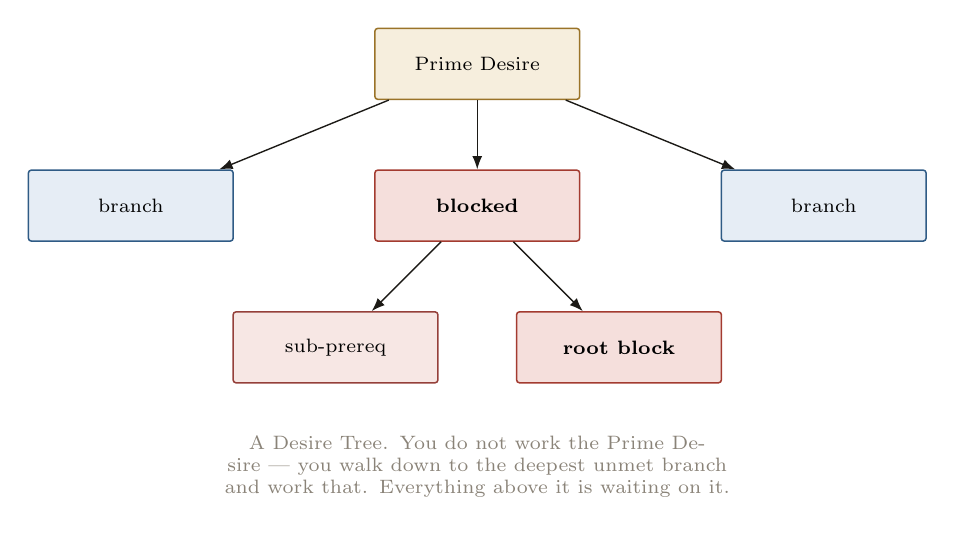
\begin{tikzpicture}[x=1mm, y=1mm, font=\sffamily\footnotesize,
  n/.style={rounded corners=1pt, minimum width=26mm, minimum height=9mm,
            draw, line width=0.55pt, align=center, font=\scriptsize},
  blocked/.style={n, fill=tksEfill, draw=tksEedge}]
  \node[n, fill=tksAfill, draw=tksAedge] (root) at (44,0) {Prime Desire};
  \node[n, fill=tksBfill, draw=tksBedge] (b1) at (0,-18)  {branch};
  \node[blocked]                          (b2) at (44,-18) {\textbf{blocked}};
  \node[n, fill=tksBfill, draw=tksBedge] (b3) at (88,-18) {branch};
  \foreach \b in {b1,b2,b3} {
    \draw[-{Latex[length=1.7mm]}, tksInk, line width=0.5pt] (root) -- (\b);
  }
  \node[n, fill=tksCfill, draw=tksCedge] (c1) at (26,-36) {sub-prereq};
  \node[blocked]                          (c2) at (62,-36) {\textbf{root block}};
  \draw[-{Latex[length=1.7mm]}, tksInk, line width=0.5pt] (b2) -- (c1);
  \draw[-{Latex[length=1.7mm]}, tksInk, line width=0.5pt] (b2) -- (c2);
  \node[anchor=north, text width=92mm, align=center, font=\scriptsize,
        text=tksMuted] at (44,-46)
    {A Desire Tree. You do not work the Prime Desire --- you walk down to the
     deepest unmet branch and work that. Everything above it is waiting on it.};
\end{tikzpicture}
\end{document}
